
 \input{../common}

\begin{document}
  %<*content>
  \sheet{algebra}{point-methodes-proba}{Calcul de probabilité (TS2)}
 \summary{}
 
 \textsc{Compétences que doit maîtriser le candidat :}
\begin{itemize}[label=\bf $ \ast $]
  \item  connaître le  vocabulaire de la probabilité ( univers, épreuve, événements).
  \item savoir calculer la probabilité d'un événement dans les cas d'équiprobabilité et de  non équiprobabilité.
  \item Reconnaître une probabilité conditionnelle
    \item  montrer que deux événements sont indépendants
 \item Utiliser la formule des probabilités totales
   \item Déterminer la loi de
probabilité d'une variable
aléatoire.
\item Calculer l'espérance, la
variance et l'écart-type
d'une variable aléatoire.
   \item Déterminer et représenter la
fonction de répartition d'une
variable aléatoire.
\item Reconnaître une loi binomiale
\item Connaître la formule de la
loi binomiale et l'utiliser
pour résoudre des
problèmes.
\end{itemize}
   \bigskip
   
   
   \textbf{Méthodologie}
\begin{enumerate}
\item\textbf{Équiprobabilité}\\
 Dans le cas d'un tirage << équiprobable>>, chaque événement élémentaire a la même probabilité d'apparition.\\
Dans ce cas, pour tout événement A\\

\hspace*{4cm} P(A)$=\dfrac{\text{nombre de cas favorables à  A}}{\text{nombre de cas possibles}}  $
\begin{itemize}[label=\bf $ \ast $]
  \item \textsc{Exemple}:\; Dans un supermarché, il y a 150 cartons de lait, dont 8 sont avariés. Un client prend 2 cartons au hasard. Quelle est la probabilité
qu'il soit mécontent ?
\item  \textsc{Réponse}\\Le nombre de cas possibles est le nombre de façons de choisir deux objets parmi 150, c’est-à-dire $ C_{150}^2=11175 $.\\
L'ordre dans lequel il choisit ses cartons n'a pas d'importance et les répétitions ne sont pas possibles ( il prend obligatoirement deux cartons distincts)\\
 Le nombre de cas favorables peut être obtenu de la manière suivante : le client est mécontent s'il obtient au moins un carton avarié\; $ C_8^2\times C_{142}^0+C_8^1\times C_{142}^1 $  .\\ $ \dfrac{C_8^2\times C_{142}^0+C_8^1\times C_{142}^1   }{C_{150}^2 }=\frac{1164}{11175} $.
\item \textbf{Méthode}\; Faire la distinction entre le << et >> qui correspond à $ \cap $ et le << ou >> qui correspond à $ \cup $ . Se servir de la formule :$ P(A\cup B)=P(A)+P(B)-P(A\cap B) $
\end{itemize}
\item \textbf{Calcul d'une probabilité conditionnelle}
\begin{itemize}[label=\bf $ \ast $]
\item \textbf{Méthode}\\
On applique la formule de définition :\; $ P_A(B)=P(B/A)=\dfrac{P(A\cap B)}{P(A)} $

  Les probabilités figurant sur les sous branches sont des probabilités conditionnelles. 
 
 \hspace*{3cm}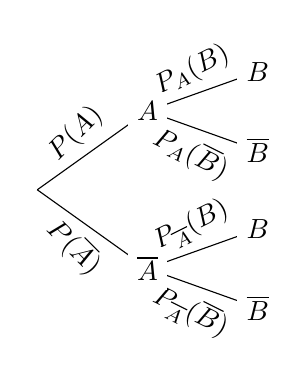
\begin{tikzpicture}[xscale=0.7,yscale=0.5]
\draw (-2,0.5)--(-4,1.5) node[midway, below, sloped]{$ P _{\overline{A}} (\overline{B})$};
 \draw (-2,2.5)--(-4,1.5) node[midway, above, sloped]{$ P _{\overline{A}} (B)  $};
 \draw (-2,4.5)--(-4,5.5) node[midway, below, sloped]{$P _{A} (\overline{B})   $};
 \draw (-2,6.5)--(-4,5.5) node[midway, above, sloped]{$ P _{A} (B) $};
 \draw (-4,1.5)--(-6,3.5) node[midway, below, sloped]{$ P(\overline{A}) $};
 \draw (-4,5.5)--(-6,3.5) node[midway, above, sloped]{$ P(A) $};
 \draw (-2,0.5) node[fill=white]{$\overline{B}$};
 \draw (-2,2.5) node[fill=white]{$B$};
 \draw (-2,4.5) node[fill=white]{$\overline{B}$};
 \draw (-2,6.5) node[fill=white]{$B$};
 \draw (-4,1.5) node[fill=white]{$\overline{A}$};
 \draw (-4,5.5) node[fill=white]{$A$};
 \end{tikzpicture}
 \item \textsc{énoncé}:\, Un sac contient trois jetons rouges et quatre jetons blancs. On en tire simultanément et hasard  deux.\\
 Calculer la probabilité pour qu'un tirage contenant un rouge contienne également un blanc?\\
 \textit{Attention à l'énoncé: il s'agit de calculer la probabilité que le tirage contient un jeton blanc sachant qu'il contient déjà un jeton rouge!}
\item \textbf{Méthode}\\
Dans l'écriture de la définition, il faut commencer par regarder ce qui conditionne.\\
Par exemple : Lors d'une compétition de tir à l'arc, on a constaté qu'un tireur entraîné a 80\% de chances d'atteindre sa cible. 80\% est la probabilité de d'atteindre la cible sous condition (sachant ) qu'on est entraîné.
\item \textbf{Formule}:\; $ P(A\cap B)=P(A/B)\times P(B)=P(B/A)\times P(A)$
\item \textsc{Exemple}:\; Lors d'une compétition de tir à l'arc, on a constaté qu'un tireur entraîné a 80 \% de chances d'atteindre sa cible. Parmi les
participants, 40 \% sont des tireurs entraînés.
Quelle est la probabilité d'être un tireur entraîné et de gagner ?\quad \textsc{réponse}:\; $ P(A\cap B)=0.8\times 0.4=0.32$
\end{itemize}
\item \textbf{Utiliser la formule des probabilités totales}
\begin{itemize}[label=\bf $ \ast $]
\item \textbf{Méthode}\\
On utilise la formule dans le cas particulier important où la partition se réduit à $ \{ A,\; \overline{A} \}. $\\
La formule devient :\; $P ( B ) = P ( B / A ) \times P ( A ) + P ( B / \overline{A} ) \times P ( \overline{A}) $.
\item\textsc{énoncé}\; Lors d'une compétition de tir à l'arc, on a constaté qu'un tireur entraîné a 80\% de chances d'atteindre sa cible. Parmi les
participants, 40 \% sont des tireurs entraînés. Les autres ont 50\% de chances d'atteindre la cible. On choisit un participant au hasard,
quelle est la probabilité qu'il atteigne la cible ?
\item \textsc{réponse}\;On désigne par A l'événement << être un tireur entraîné >> et par G l'événement << atteindre la cible>>\\`
$ P(G)=P ( G / A ) \times P ( A ) + P ( G / \overline{A} ) \times P ( \overline{A})=0.8\times 0.4+0.5\times0.6=0.62 $
\item \textbf{Indépendance deux événements}\\
 \textbf{Définition}:\quad
On dit que \textbf {les événements A et B sont indépendants} si,\quad 
$ P(A\cap B)= P(A)\times  P(B)$
\item\textsc{Propriété}:\;
A et B sont indépendants si, et seulement si, P$_{A}(B)=P(B) $\; ou\; P$ _{B}(A)=P(A) $.

\end{itemize}
\item \textbf{Etude d'une variable aléatoire}\\
Déterminer une loi de probabilité\\
\textbf{Méthode}
\begin{itemize}[label=\bf $ \bullet $]
\item première étape : regarder les valeurs que peut prendre la variable aléatoire X ;
\item deuxième étape : regarder ce que signifie chacun des événements ;
\item  troisième étape : calculer les probabilités de chacun des événements déterminés précédemment.\\
On peut utiliser un tableau  pour représenter la loi de probabilité.

 $\begin{array}{|c|c|c|c|c|c|}
\hline
  x_{i} &  x_1 &  x_2 & ... &  x_n \\
\hline
 P(X=x_{i})  &  p_1 &  p_2    & ...&  p_n \\
\hline
\end{array}$

\textbf{NB}: \quad  on a\quad $  p_1 + p_2+ ... +p_n = 1$
\end{itemize}
\item \textbf{ Espérance mathématique}\\
L'espérance mathématique de X notée E(X) , est  définie par :\; E(X)$ = p_1 x_1 + p_2 x_2 +... + p_n x_n$.
\item \textbf{  Variance et écart type}\\
La variance de X, notée $V(X)$ est  définie par: $  V(X) = E(X^2 ) - (E(X))^2 $.\\
L'écart type de X, noté  $ \sigma $ est \quad  $ \sigma=\sqrt{V(X)} $.  
\item \textbf{Déterminer une fonction de répartition}\\
\textbf{Méthode}\\
Il suffit d'appliquer la définition  $F (x ) = P ( X \leq x ) $.\\
Pour calculer cette probabilité, il faut << cumuler  les valeurs>>.

\item \textbf{Reconnaître une loi binomiale}\\
\textbf{Méthode}\\
Il faut repérer l'épreuve de Bernoulli, déterminer la valeur de p (probabilité de succès à une épreuve de Bernoulli). Puis déterminer
la valeur de $ n $ , nombre de fois où cette épreuve de Bernoulli est répétée (épreuves indépendantes).\\
\textbf{Loi binomiale}\\
La loi de probabilité correspondant à un schéma de Bernoulli est appelée \textbf{loi binomiale de
paramètre} $ n $ et $ p $, c'est-à-dire pour tout entier $ k $ de $[0 ; n]$ on a : P$ (X=k)=C_{n}^{k}p^{k}(1-p)^{n-k} $

\smallskip
L'espérance mathématique de X est E(X)$ =np $ et la variance V(X)$=np(1-p)  $\\

\textsc{Exemple:}\ Lors d'une compétition de tir à l'arc, on a constaté qu'un tireur entraîné a 80 \% de chances d'atteindre sa cible. Parmi les
participants, 40 \% sont des tireurs entraînés. Les autres ont 50\% de chances d'atteindre la cible.\\
On choisit un tireur au hasard, on lui fait faire 10 tirs consécutifs, indépendants.\\
Calculer la probabilité qu'il atteigne exactement 7 fois la cible.\\


\hspace*{3cm}\; $ P(X=7)=C_{10}^7(0.62)^7(1-0.62)^3=0.2319 $
\end{enumerate}
\end{document}